% Todo Management Application — System Documentation
% Compile: pdflatex main.tex (run twice for TOC/refs)
%
% Structure:
%   module/frontmatter.tex   — document control (revision history)
%   module/overview.tex      — project-wide context
%   module/phase01.tex … phase05.tex — one file per SDLC phase (each opens with \PhaseTitlePage)
\documentclass{article}
\hbadness=10000
\vbadness=10000

% -------------------------------------------------------------------
% PACKAGES
% -------------------------------------------------------------------
\usepackage[utf8]{inputenc}
\usepackage[T1]{fontenc}
\usepackage{lmodern}
\usepackage[english]{babel}
\usepackage[margin=1in]{geometry}
\usepackage{parskip}
\usepackage{graphicx}
\usepackage[table]{xcolor} 
\usepackage{colortbl}
\usepackage{tikz}
\usetikzlibrary{shapes,shapes.multipart,arrows,positioning,fit,backgrounds,shadows,arrows.meta,calc,babel}
\usepackage{tabularx}
\usepackage{booktabs}
\usepackage{array}
\usepackage{enumitem}
\usepackage{amssymb}
\usepackage{listings}
\usepackage{fancyhdr}
\pagestyle{fancy}
\fancyhf{}
\fancyhead[L]{Todo Management Application \textbar\ \nouppercase{\leftmark}}
\fancyfoot[C]{\thepage}
\renewcommand{\headrulewidth}{0.4pt}
\usepackage{hyperref}
\hypersetup{
  colorlinks=true,
  linkcolor=blue,
  urlcolor=blue,
  pdftitle={Todo Management Application — System Documentation},
  pdfauthor={The DJs}
}
\lstset{
  basicstyle=\ttfamily\small,
  breaklines=true,
  columns=fullflexible,
  showstringspaces=false
}

% Update running header (call after each \section or at document start)
\newcommand{\SetDocHeader}[1]{\markboth{#1}{#1}}

% -------------------------------------------------------------------
% Per-phase title page (each module calls this once at the top)
% -------------------------------------------------------------------
% Usage: \PhaseTitlePage{<n>}{<phase name>}{<doc id>}{<document type>}
% Example: \PhaseTitlePage{1}{Requirements Analysis}{TMA-RAD-P1}{Requirements Analysis Document}
% Do not use the titlepage environment --- it resets \thepage to 1 each time.
% Scope layout in a group so \centering does not leak into body content.
\newcommand{\PhaseTitlePage}[4]{%
  \clearpage
  \thispagestyle{empty}%
  \begingroup
  \centering
  \vspace*{2.5cm}
  {\large\textit{#4}\par}
  \vspace{1.2cm}
  {\Huge\bfseries Todo Management Application\par}
  \vspace{0.5cm}
  {\large Revature --- Full-Stack SDLC Project\par}
  \vspace{0.8cm}
  {\Large Phase #1: #2\par}
  \vspace{2.5cm}
  {\large\textbf{The DJs}\par}
  \vspace{1.5cm}
  \begin{tabular}{@{}c@{}}
    \toprule
    \textbf{Prepared by} \\
    \midrule
    Jaehoon Song \\
    Daniel Patience \\
    Jacqueline Lainhart \\
    \bottomrule
  \end{tabular}
  \vfill
  \begin{minipage}{0.72\textwidth}
    \centering
    \begin{tabular}{@{}r@{\hspace{1.2em}}l@{}}
      \textbf{Document ID:} & #3 \\
      \textbf{Version:}    & 0.1 \\
      \textbf{Status:}     & Draft \\
      \textbf{Phase:}      & #1 of 5 \\
      \textbf{Issue date:}  & \today \\
    \end{tabular}
  \end{minipage}
  \vspace{2cm}
  \par
  \endgroup
  \clearpage
}







% Raw HTTP/JSON payloads (CS-A: rest.tex). Framed listings pair with httpexchange below.
\lstdefinestyle{http}{%
  basicstyle=\ttfamily\footnotesize,
  frame=single,
  framerule=0.4pt,
  framesep=3pt,
  xleftmargin=2pt,
  xrightmargin=2pt,
  breaklines=true,
  breakatwhitespace=true,
  columns=fullflexible,
  keepspaces=true,
  aboveskip=4pt,
  belowskip=4pt,
}
\lstnewenvironment{httplisting}{\lstset{style=http}}{}

% Side-by-side request/response. One tabular row; \httpmidarrows sits between listings.
% Do not pass lstlisting through a macro argument.
\tikzset{%
  http@arrow/.style={%
    -{Stealth[scale=0.88]}, semithick, shorten >=0.5pt, shorten <=0.5pt, draw=black!55},
}
\newenvironment{httpexchange}{%
  \par\medskip
  \begingroup
  \hfuzz=30pt\relax
  \begin{center}%
  \noindent
  \begin{tabular}{@{} m{0.4\linewidth} >{\centering\arraybackslash}m{1.28cm} m{0.4\linewidth} @{}}%
}{%
  \end{tabular}%
  \end{center}%
  \endgroup
  \medskip
}
\newcommand{\httpmidarrows}{%
  &
  \begin{minipage}[c]{1.28cm}%
    \centering
    \normalfont\footnotesize REQ\par\vspace{1pt}%
    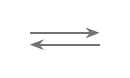
\begin{tikzpicture}[x=1cm, y=0.75cm]
      \draw[http@arrow] (0,0.1) -- (0.92,0.1);
      \draw[http@arrow] (0.92,-0.1) -- (0,-0.1);
    \end{tikzpicture}\par\vspace{1pt}%
    \normalfont\footnotesize RESP%
  \end{minipage}%
  &
}









% -------------------------------------------------------------------
\begin{document}
% -------------------------------------------------------------------

% Document control (IEEE 830 / ISO front matter).
% Per-phase title pages are issued via \PhaseTitlePage in each phase module.

\SetDocHeader{Todo Management Application}
\thispagestyle{empty}
\begin{center}
  {\LARGE\bfseries Todo Management Application\par}
  \vspace{0.4cm}
  {\large Revature --- Full-Stack SDLC Project\par}
  \vspace{0.3cm}
  {\large System Documentation\par}
  \vspace{0.3cm}
  {\large\textbf{The DJs}\par}
\end{center}

\vspace{1cm}
\begin{center}
  \begin{tabular}{@{}c@{}}
    \toprule
    \textbf{Prepared by} \\
    \midrule
    Jaehoon Song \\
    Daniel Patience \\
    Jacqueline Lainhart \\
    \bottomrule
  \end{tabular}
\end{center}

\vspace{1.5cm}
\begin{center}
  {\large\bfseries Document Control}
\end{center}
\vspace{0.5cm}
\subsection*{Revision History}
Per IEEE~830 and ISO document-control practice, all revisions are recorded below.

\vspace{0.4cm}
\begin{tabularx}{\textwidth}{@{} c c l X @{}}
  \toprule
  \textbf{Version} & \textbf{Date} & \textbf{Author} & \textbf{Description} \\
  \midrule
  0.1 & \today & The DJs & Initial draft --- Phases 1--5 system documentation \\
  \bottomrule
\end{tabularx}

\vspace{1.2cm}
\subsection*{Document Information}
\begin{tabularx}{\textwidth}{@{} l X @{}}
  \toprule
  \textbf{Field} & \textbf{Value} \\
  \midrule
  Document type     & System Documentation (5-phase SDLC) \\
  Organization      & Revature \\
  Project           & Todo Management Application --- Full-Stack SDLC \\
  Team              & The DJs \\
  Authors           & Jaehoon Song, Daniel Patience, Jacqueline Lainhart \\
  Intended audience & Development team and Revature instructors (Trainers) \\
  Module structure  & \texttt{modules/phase01.tex} through \texttt{phase05.tex} \\
  \bottomrule
\end{tabularx}

\newpage

\tableofcontents

\newpage
% Project-wide context — included once before phase modules.

\section{Project Overview}\label{sec:overview}
\SetDocHeader{Project Overview}

\subsection{Objective}
Build a full-stack, secure Todo Management application as part of the Revature full-stack
SDLC training program. The team moves from initial requirement analysis to a functional
product demonstration, simulating a real-world Software Development Lifecycle (SDLC).

\subsection{Technology Stack}
\begin{tabularx}{\textwidth}{@{} l X @{}}
\toprule
\textbf{Layer} & \textbf{Technology} \\
\midrule
Frontend       & Angular \\
Backend        & Java (Spring Boot, Web, Data JPA) \\
Database       & SQLite \\
Build / Tools  & Gradle, Git, GitHub \\
\bottomrule
\end{tabularx}

\subsection{User Stories (Scope)}
The following stories define \emph{what} the system must deliver. Each phase builds on
the prior phase toward a complete implementation.

\begin{enumerate}
  \item \textbf{Registration:} As a new user, I can register an account.
  \item \textbf{Authentication:} As a user, I can log in and log out securely.
  \item \textbf{Task Management:} As a user, I can create, read, update, and delete primary Todo items.
  \item \textbf{Organization:} As a user, I can create, read, update, and delete nested subtasks.
\end{enumerate}

\subsection{Project Roadmap}
\begin{tabularx}{\textwidth}{@{} c l X @{}}
\toprule
\textbf{Phase} & \textbf{Name} & \textbf{Goal} \\
\midrule
1 & Requirements Analysis & Deconstruct user stories; define schema and API contracts. \\
2 & Design                & Plan architecture, wireframes, and security flows. \\
3 & Backend Development   & Build REST API, security layer, and persistence. \\
4 & Frontend Development  & Build Angular UI and integrate with the API. \\
5 & Presentation          & Demonstrate working software and architecture. \\
\bottomrule
\end{tabularx}

\newpage

% Phase 1: Requirements Analysis

\PhaseTitlePage{1}{Requirements Analysis}{TMA-RAD-P1}{Requirements Analysis Document}

\section{Phase 1: Requirements Analysis}\label{sec:phase1}
\SetDocHeader{Phase 1: Requirements Analysis}

\subsection{Objective}
The goal of this phase is the technical decomposition of user stories. Before any code is written,
the team must define the data structures, the API communication standards, and the criteria for
successful completion.

\subsubsection{Checkpoints}
\begin{itemize}
  \item[$\square$] \textbf{Task Breakdown:} Deconstruct user stories into granular technical tasks.
  \item[$\square$] \textbf{Database Modeling:} Design the relational schema (User, Todo, and Subtask entities).
  \item[$\square$] \textbf{API Contract:} Define RESTful endpoints and expected JSON request/response bodies.
  \item[$\square$] \textbf{Definition of Done (DoD):} Establish team-specific criteria for completed work.
\end{itemize}

\subsubsection{Technical Reference: User Stories}
Use these stories as the foundation for your task breakdown and API design:
\begin{enumerate}
  \item \textbf{Account Creation:} As a new user, I can register an account to start tracking my todo tasks.
  \item \textbf{Authentication:} As a new user, I can log in and out to securely access my todo items.
  \item \textbf{Task Management:} As a user, I can create, edit, and delete todo items to keep track of my work.
  \item \textbf{Subtask Organization:} As a user, I can create, edit, and delete subtask items to better organize my primary tasks.
\end{enumerate}

\subsubsection{Deliverables for Phase 1}
By the end of this phase, your team should have a shared document or repository folder containing:
\begin{enumerate}
  \item \textbf{Entity Relationship Diagram (ERD):} Visual or text-based representation of your SQLite schema.
  \item \textbf{API Specification:} A list of endpoints (e.g., \texttt{POST /api/auth/register}, \texttt{GET /api/todos}) including expected payloads.
  \item \textbf{Task Backlog:} A list of specific, actionable items ready to be assigned to team-members.
  \begin{itemize}
    \item Use GitHub Issues and Github Project to facilitate this.
  \end{itemize}
\end{enumerate}

\subsubsection{Moving to Phase 2}
Once all Phase~1 checkboxes are marked as complete and the team agrees on the API contracts,
proceed to \textbf{Phase 2: Design}.








\newpage
\subsection{Task Breakdown}\label{sec:tasks}

\subsubsection{Epic 1: Account Creation}
\textbf{User story:} As a new user, I can register an account to start tracking my todo tasks.

\begin{tabularx}{\textwidth}{@{} p{2.4cm} X @{}}
\toprule
\textbf{Task ID} & \textbf{Description} \\
\midrule 
AUTH-01 & Define \texttt{User} entity fields (id, username, email, password); SQLite \texttt{users} table. \\
AUTH-02 & Encrypt passwords before storage (persist hash only, never plaintext). \\
AUTH-03 & Define validation rules (unique username/email, required fields). \\
AUTH-04 & Specify registration endpoint: \texttt{POST /api/auth/register}. \\
AUTH-05 & Document responses: HTTP 200 on success; HTTP 409 duplicate username/email; HTTP 400 on validation errors. \\
\bottomrule
\end{tabularx}

\subsubsection{Epic 2: Authentication}
\textbf{User story:} As a user, I can log in and log out to securely access my todo items.

\begin{tabularx}{\textwidth}{@{} p{2.4cm} X @{}}
\toprule
\textbf{Task ID} & \textbf{Description} \\
\midrule
AUTH-06 & Verify username/password combination against the database on login. \\
AUTH-07 & Specify login endpoint: \texttt{POST /api/auth/login}. \\
AUTH-08 & Return HTTP 200 when request JSON matches stored credentials. \\
AUTH-09 & Define session-based authentication for protected routes. \\
AUTH-10 & Document logout behavior and HTTP 401 responses for unauthenticated access. \\
\bottomrule
\end{tabularx}

\subsubsection{Epic 3: Task Management}
\textbf{User story:} As a user, I can create, edit, and delete todo items to keep track of my work.

\begin{tabularx}{\textwidth}{@{} p{2.4cm} X @{}}
\toprule
\textbf{Task ID} & \textbf{Description} \\
\midrule
TODO-01 & Define \texttt{Todo} entity (id, title, description, completed, user\_id, timestamps). \\
TODO-02 & Specify \texttt{POST /api/todos} --- create todo. \\
TODO-03 & Specify \texttt{GET /api/todos} --- list todos for authenticated user. \\
TODO-04 & Specify \texttt{GET /api/todos/\{id\}} --- retrieve single todo. \\
TODO-05 & Specify \texttt{PUT /api/todos/\{id\}} --- update todo fields. \\
TODO-06 & Specify \texttt{DELETE /api/todos/\{id\}} --- delete todo (cascade subtasks). \\
TODO-07 & Enforce ownership: users may only access their own todos. \\
\bottomrule
\end{tabularx}

\subsubsection{Epic 4: Subtask Organization}
\textbf{User story:} As a user, I can create, edit, and delete subtask items to better organize my primary tasks.

\begin{tabularx}{\textwidth}{@{} p{2.4cm} X @{}}
\toprule
\textbf{Task ID} & \textbf{Description} \\
\midrule
SUB-01 & Define \texttt{Subtask} entity (id, title, completed, todo\_id, timestamps). \\
SUB-02 & Use \texttt{GET /api/todos/\{id\}} to retrieve the parent todo before subtask operations. \\
SUB-03 & Specify \texttt{POST /api/todos/\{id\}/\{subtask\}} --- create subtask. \\
SUB-04 & Specify \texttt{PATCH /api/todos/\{id\}/\{subtask\}} --- update subtask fields. \\
SUB-05 & Specify \texttt{DELETE /api/todos/\{id\}/\{subtask\}} --- delete subtask. \\
SUB-06 & Validate parent todo exists, belongs to the authenticated user; document cascade delete when parent todo is removed. \\
\bottomrule
\end{tabularx}

\newpage
\subsection{Database Modeling}\label{sec:database}

\subsubsection{Entity Summary}
\begin{tabularx}{\textwidth}{@{} l l X @{}}
\toprule
\textbf{Entity} & \textbf{Table} & \textbf{Purpose} \\
\midrule
User    & \texttt{users}    & Account credentials and identity \\
Todo    & \texttt{todos}    & Primary task items owned by a user \\
Subtask & \texttt{subtasks} & Nested items belonging to one todo \\
\bottomrule
\end{tabularx}

\subsubsection{Entity Relationship Diagram}
Figure~\ref{fig:erd} shows a compact \textbf{Crow's Foot} (IE) style ERD.
Each \texttt{todo} references exactly one \texttt{user} (\texttt{user\_id});
each \texttt{user} owns zero or more \texttt{todos}.
Each \texttt{subtask} references exactly one \texttt{todo} (\texttt{todo\_id});
each \texttt{todo} has zero or more \texttt{subtasks}.

\begin{figure}[htbp]
  \centering
  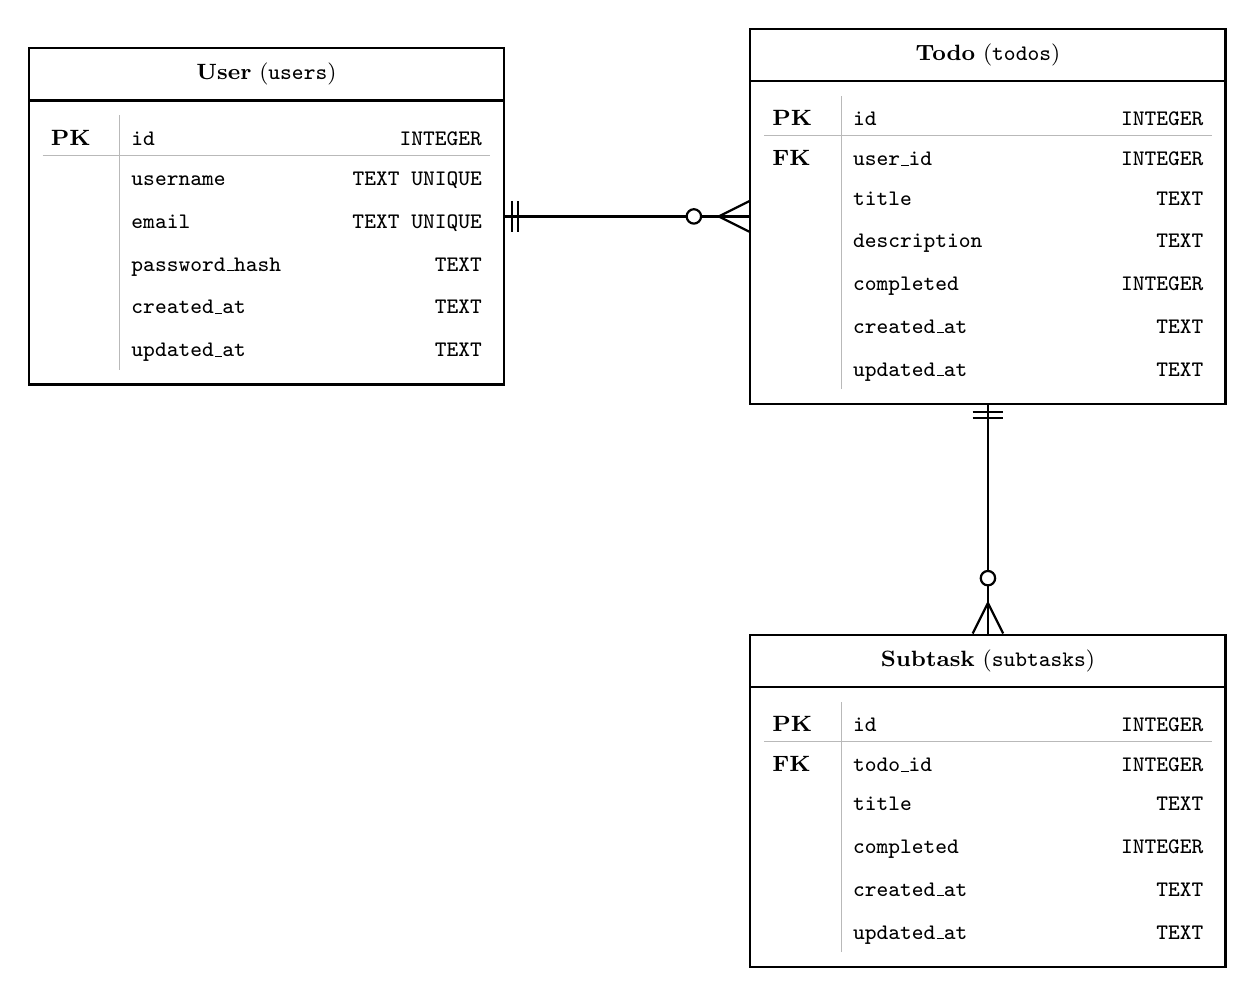
\begin{tikzpicture}[
    font=\footnotesize,
    entity/.style={
      rectangle split,
      rectangle split parts=2,
      draw,
      thick,
      minimum width=5.9cm,
      inner sep=5pt,
      rectangle split part align={center, left},
    },
  ]
    \node[entity] (User) {
      \textbf{User} {\footnotesize(\texttt{users})}
      \nodepart{two}
      {\setlength{\tabcolsep}{2pt}%
       \setlength{\extrarowheight}{2.5pt}%
       \renewcommand{\arraystretch}{1.18}%
       \begin{tabular}{@{\hspace{3pt}}p{8mm}!{\color{gray!55}\vrule width 0.35pt}@{\hspace{4pt}}p{4.45cm}@{\hspace{3pt}}}
        \textbf{PK} & \texttt{id}\hfill\texttt{INTEGER}\\
        \arrayrulecolor{gray!55}\hline\arrayrulecolor{black}
         & \texttt{username}\hfill\texttt{TEXT UNIQUE}\\
         & \texttt{email}\hfill\texttt{TEXT UNIQUE}\\
         & \texttt{password\_hash}\hfill\texttt{TEXT}\\
         & \texttt{created\_at}\hfill\texttt{TEXT}\\
         & \texttt{updated\_at}\hfill\texttt{TEXT}\\
       \end{tabular}%
      }
    };

    \node[entity, right=3.1cm of User] (Todo) {
      \textbf{Todo} {\footnotesize(\texttt{todos})}
      \nodepart{two}
      {\setlength{\tabcolsep}{2pt}%
       \setlength{\extrarowheight}{2.5pt}%
       \renewcommand{\arraystretch}{1.18}%
       \begin{tabular}{@{\hspace{3pt}}p{8mm}!{\color{gray!55}\vrule width 0.35pt}@{\hspace{4pt}}p{4.45cm}@{\hspace{3pt}}}
        \textbf{PK} & \texttt{id}\hfill\texttt{INTEGER}\\
        \arrayrulecolor{gray!55}\hline\arrayrulecolor{black}
        \textbf{FK} & \texttt{user\_id}\hfill\texttt{INTEGER}\\
         & \texttt{title}\hfill\texttt{TEXT}\\
         & \texttt{description}\hfill\texttt{TEXT}\\
         & \texttt{completed}\hfill\texttt{INTEGER}\\
         & \texttt{created\_at}\hfill\texttt{TEXT}\\
         & \texttt{updated\_at}\hfill\texttt{TEXT}\\
       \end{tabular}%
      }
    };

    \node[entity, below=2.9cm of Todo] (Subtask) {
      \textbf{Subtask} {\footnotesize(\texttt{subtasks})}
      \nodepart{two}
      {\setlength{\tabcolsep}{2pt}%
       \setlength{\extrarowheight}{2.5pt}%
       \renewcommand{\arraystretch}{1.18}%
       \begin{tabular}{@{\hspace{3pt}}p{8mm}!{\color{gray!55}\vrule width 0.35pt}@{\hspace{4pt}}p{4.45cm}@{\hspace{3pt}}}
        \textbf{PK} & \texttt{id}\hfill\texttt{INTEGER}\\
        \arrayrulecolor{gray!55}\hline\arrayrulecolor{black}
        \textbf{FK} & \texttt{todo\_id}\hfill\texttt{INTEGER}\\
         & \texttt{title}\hfill\texttt{TEXT}\\
         & \texttt{completed}\hfill\texttt{INTEGER}\\
         & \texttt{created\_at}\hfill\texttt{TEXT}\\
         & \texttt{updated\_at}\hfill\texttt{TEXT}\\
       \end{tabular}%
      }
    };

    % User (one) --- (many) Todo  [horizontal]
    \coordinate (TodoWest) at (Todo.west);
    \coordinate (CrowUT) at ($(TodoWest)+(-11pt,0)$);
    \coordinate (RingUT) at ($(CrowUT)+(-9pt,0)$);
    \coordinate (UserEast) at (User.east);
    \coordinate (PipeUT) at ($(UserEast)+(2.4pt,0)$);
    \draw[thick] (UserEast) -- ($(RingUT)+(-2.6pt,0)$);
    \draw[thick] (RingUT) circle[radius=2.6pt];
    \draw[thick] ($(RingUT)+(2.6pt,0)$) -- (CrowUT);
    \draw[thick] ($(PipeUT)+(0,5.5pt)$) -- ($(PipeUT)+(0,-5.5pt)$);
    \draw[thick] ($(PipeUT)+(2.3pt,5.5pt)$) -- ($(PipeUT)+(2.3pt,-5.5pt)$);
    \draw[thick] (CrowUT) -- ($(TodoWest)+(0,5.5pt)$);
    \draw[thick] (CrowUT) -- (TodoWest);
    \draw[thick] (CrowUT) -- ($(TodoWest)+(0,-5.5pt)$);

    % Todo (one) --- (many) Subtask  [vertical]
    \coordinate (SubNorth) at (Subtask.north);
    \coordinate (CrowTS) at ($(SubNorth)+(0,11pt)$);
    \coordinate (RingTS) at ($(CrowTS)+(0,9pt)$);
    \coordinate (TodoSouth) at (Todo.south);
    \coordinate (PipeTS) at ($(TodoSouth)+(0,-2.4pt)$);
    \draw[thick] (TodoSouth) -- ($(RingTS)+(0,2.6pt)$);
    \draw[thick] (RingTS) circle[radius=2.6pt];
    \draw[thick] ($(RingTS)+(0,-2.6pt)$) -- (CrowTS);
    \draw[thick] ($(PipeTS)+(-5.5pt,0)$) -- ($(PipeTS)+(5.5pt,0)$);
    \draw[thick] ($(PipeTS)+(-5.5pt,-2.3pt)$) -- ($(PipeTS)+(5.5pt,-2.3pt)$);
    \draw[thick] (CrowTS) -- ($(SubNorth)+(-5.5pt,0)$);
    \draw[thick] (CrowTS) -- (SubNorth);
    \draw[thick] (CrowTS) -- ($(SubNorth)+(5.5pt,0)$);
  \end{tikzpicture}
  \caption{Crow's Foot ERD}
  \label{fig:erd}
\end{figure}

\newpage

\subsubsection{Data Dictionary}
The ERD above is the canonical model. Table~\ref{tab:data-dictionary} maps each logical
entity to its SQLite columns, types, and constraints.

\begin{table}[htbp]
  \centering
  \caption{SQLite data dictionary}
  \label{tab:data-dictionary}
  \small
  \begin{tabularx}{\textwidth}{@{} l l l X @{}}
    \toprule
    \textbf{Table} & \textbf{Column} & \textbf{Type} & \textbf{Constraints / Notes} \\
    \midrule
    \texttt{users} & \texttt{id}             & \texttt{INTEGER} & \texttt{PRIMARY KEY}, \texttt{AUTOINCREMENT} \\
    \texttt{users} & \texttt{username}       & \texttt{TEXT}    & \texttt{NOT NULL}, \texttt{UNIQUE} \\
    \texttt{users} & \texttt{email}          & \texttt{TEXT}    & \texttt{NOT NULL}, \texttt{UNIQUE} \\
    \texttt{users} & \texttt{password\_hash} & \texttt{TEXT}    & \texttt{NOT NULL} \\
    \texttt{users} & \texttt{created\_at}    & \texttt{TEXT}    & \texttt{NOT NULL}; ISO-8601 timestamp \\
    \texttt{users} & \texttt{updated\_at}    & \texttt{TEXT}    & \texttt{NOT NULL}; ISO-8601 timestamp \\
    \midrule
    \texttt{todos} & \texttt{id}             & \texttt{INTEGER} & \texttt{PRIMARY KEY}, \texttt{AUTOINCREMENT} \\
    \texttt{todos} & \texttt{user\_id}       & \texttt{INTEGER} & \texttt{NOT NULL}; \texttt{REFERENCES} \texttt{users(id)}, \texttt{ON DELETE CASCADE} \\
    \texttt{todos} & \texttt{title}          & \texttt{TEXT}    & \texttt{NOT NULL} \\
    \texttt{todos} & \texttt{description}    & \texttt{TEXT}    & Optional \\
    \texttt{todos} & \texttt{completed}      & \texttt{INTEGER} & \texttt{NOT NULL}, \texttt{DEFAULT} \texttt{0} (\texttt{0} = false, \texttt{1} = true) \\
    \texttt{todos} & \texttt{created\_at}    & \texttt{TEXT}    & \texttt{NOT NULL}; ISO-8601 timestamp \\
    \texttt{todos} & \texttt{updated\_at}    & \texttt{TEXT}    & \texttt{NOT NULL}; ISO-8601 timestamp \\
    \midrule
    \texttt{subtasks} & \texttt{id}          & \texttt{INTEGER} & \texttt{PRIMARY KEY}, \texttt{AUTOINCREMENT} \\
    \texttt{subtasks} & \texttt{todo\_id}    & \texttt{INTEGER} & \texttt{NOT NULL}; \texttt{REFERENCES} \texttt{todos(id)}, \texttt{ON DELETE CASCADE} \\
    \texttt{subtasks} & \texttt{title}       & \texttt{TEXT}    & \texttt{NOT NULL} \\
    \texttt{subtasks} & \texttt{completed}   & \texttt{INTEGER} & \texttt{NOT NULL}, \texttt{DEFAULT} \texttt{0} \\
    \texttt{subtasks} & \texttt{created\_at} & \texttt{TEXT}    & \texttt{NOT NULL}; ISO-8601 timestamp \\
    \texttt{subtasks} & \texttt{updated\_at} & \texttt{TEXT}    & \texttt{NOT NULL}; ISO-8601 timestamp \\
    \bottomrule
  \end{tabularx}
\end{table}

\subsubsection{Integrity Rules}
\begin{itemize}
  \item \texttt{users.username} and \texttt{users.email} must be unique.
  \item Every \texttt{todo} must reference a valid \texttt{user\_id}.
  \item Every \texttt{subtask} must reference a valid \texttt{todo\_id}.
  \item Deleting a user cascades to their todos and subtasks.
  \item Deleting a todo cascades to its subtasks.
\end{itemize}

\newpage
\subsection{API Contract}\label{sec:api}
Define RESTful endpoints with JSON request/response bodies and expected HTTP status codes.
See deliverable checklist in Section~\ref{sec:phase1}.

\newpage
\subsection{Definition of Done}\label{sec:dod}
Establish team-specific criteria for completed work before moving to Phase~2.
See deliverable checklist in Section~\ref{sec:phase1}.

\newpage

% Phase 2: Design

\PhaseTitlePage{2}{Design}{TMA-DES-P2}{Design Document}

\section{Phase 2: Design}\label{sec:phase2}
\SetDocHeader{Phase 2: Design}

\subsection{Objective}
The goal of this phase is architectural and interface planning. The team must define the data flow,
security protocols, and user interface layouts. Successful completion of this phase ensures that
the Backend and Frontend teams can work in parallel without integration conflicts.

\subsubsection{Checkpoints}
\begin{itemize}
  \item[$\square$] \textbf{System Architecture:} Document the data flow (Angular $\rightarrow$ Spring Boot $\rightarrow$ SQLite).
  \item[$\square$] \textbf{Security Planning:} Familiarize yourself with JJWT.
  \item[$\square$] \textbf{UI Wireframing:} Map out the interface for authentication and task management.
  \item[$\square$] \textbf{Component Design:} Loosely define the Angular component hierarchy and service structure.
\end{itemize}

\subsection{Technical Reference: Design Standards}

\subsubsection{API Design Principles}
All endpoints must follow RESTful conventions. Use the following templates for your design documentation:

\subsubsection{Resource Creation Flow (Template)}
Use this logic to design your \texttt{POST} endpoints to ensure consistent error handling
(e.g., handling duplicate entries).
\begin{enumerate}[label=\arabic*., nosep, leftmargin=*]
  \item Client/Requester sends a Create Request to the API/Interface Layer.
  \item API forwards the request to the Business Logic Layer for processing.
  \item[\textbf{A.}] Resource is unique: Logic checks existence via Data Access $\rightarrow$ Storage (not found); persists the new resource; returns a 2xx Success Response to the client.
  \item[\textbf{B.}] Conflict / already exists: Logic checks existence (found); signals conflict to API; returns a 4xx Error Response to the client.
\end{enumerate}

\subsubsection{Login/Auth Flow (Template)}
Use this logic to design your \texttt{/auth} endpoints to ensure secure credential validation.
\begin{enumerate}[label=\arabic*., nosep, leftmargin=*]
  \item Client/Requester sends a Login Request to the API/Interface Layer.
  \item API forwards the request to the Business Logic Layer.
  \item[\textbf{A.}] Success: Logic fetches user data via Data Access $\rightarrow$ Storage; Utility validates credentials and generates a token; API returns a 2xx Success Response with token.
  \item[\textbf{B.}] Invalid credentials: Logic fetches user data (null/empty); API returns a 4xx Error Response to the client.
\end{enumerate}

\subsubsection{Deliverables for Phase 2}
By the end of this phase, your team should have:
\begin{enumerate}
  \item \textbf{API Specification:} A completed document defining all endpoints, request bodies, and response codes.
  \item \textbf{Wireframes:} Visual mockups of the Login, Register, and Dashboard screens.
  \item \textbf{Database Schema:} A final relational model (ERD) ready for implementation.
\end{enumerate}

\subsubsection{Moving to Phase 3}
Once the API contracts and UI wireframes are finalized and agreed upon by all team members,
proceed to \textbf{Phase 3: Backend Development}.

\newpage

\input{module/phase03}
% Phase 4: Frontend Development

\PhaseTitlePage{4}{Frontend Development}{TMA-FE-P4}{Frontend Development Document}

\section{Phase 4: Frontend Development}\label{sec:phase4}
\SetDocHeader{Phase 4: Frontend Development}

\subsection{Objective}
The goal of this phase is to build a responsive and interactive user interface. This phase focuses on
the ``interface'' of the application: consuming the Spring Boot API, managing user authentication
state via JWT, and creating a seamless user experience for task management.

\subsubsection{Checkpoints}
\begin{itemize}
  \item[$\square$] \textbf{Project Scaffolding:} Initialize Angular and configure environment settings.
  \item[$\square$] \textbf{Service Layer:} Build Angular services to consume the Spring Boot API.
  \item[$\square$] \textbf{Auth Integration:} Implement login/register forms and JWT-based state management.
  \item[$\square$] \textbf{Task Management UI:} Build the dashboard, task creation forms, and subtask nested lists.
  \item[$\square$] \textbf{Design Validation:} Confirm the UI components and user workflows match the Phase~2 wireframes.
\end{itemize}

\subsection{Technical Requirements}

\subsubsection{Authentication \& JWT Handling}
\begin{itemize}
  \item \textbf{Token Storage:} Securely store the JWT (e.g., in \texttt{localStorage} or a state management store) upon successful login.
  \item \textbf{Interceptors:} Implement an Angular \texttt{HttpInterceptor} to automatically attach the \texttt{Authorization: Bearer <token>} header to all outgoing API requests.
  \item \textbf{Route Guards:} Implement \texttt{CanActivate} guards to prevent unauthenticated users from accessing the Task Dashboard.
  \item \textbf{Logout Logic:} Implement a clear logout flow that clears the token and redirects the user to the login page.
\end{itemize}

\subsubsection{API Integration}
\begin{itemize}
  \item \textbf{Asynchronous Operations:} Use RxJS Observables to handle all API calls to ensure the UI remains responsive during data fetching.
  \item \textbf{Error Handling:} Implement user-friendly error messages (e.g., ``Invalid credentials'' or ``Task not found'') based on the HTTP status codes returned by the backend.
\end{itemize}

\subsubsection{User Interface (UI)}
\begin{itemize}
  \item \textbf{Responsiveness:} Ensure the layout is functional across different screen sizes.
  \item \textbf{Component Hierarchy:} Follow the component structure defined during the Phase~2 design to maintain code modularity.
\end{itemize}

\subsubsection{Deliverables for Phase 4}
By the end of this phase, your team should have:
\begin{enumerate}
  \item \textbf{Functional Angular Application:} A complete, running frontend integrated with the backend.
  \item \textbf{End-to-End Workflow:} A user can successfully register, log in, manage todos, and manage subtasks without errors.
  \item \textbf{Verified UI/UX:} A UI that matches the wireframes and provides a smooth, intuitive user experience.
\end{enumerate}

\subsubsection{Moving to Phase 5}
Once the frontend is fully integrated and all user stories are functional,
proceed to \textbf{Phase 5: Presentation}.

\newpage

% Phase 5: Presentation

\PhaseTitlePage{5}{Presentation}{TMA-PRES-P5}{Presentation Document}

\section{Phase 5: Presentation}\label{sec:phase5}
\SetDocHeader{Phase 5: Presentation}

\subsection{Objective}
The goal of this phase is the formal demonstration of project completion. The team must prove that
the application meets the original user stories, functions reliably, and was developed using
professional software engineering standards.

\subsection{Checkpoints}
\begin{itemize}
  \item[$\square$] \textbf{Functional Demo:} Perform a complete walkthrough of all user stories in a live environment.
  \item[$\square$] \textbf{Technical Review:} Explain the architectural choices, including the Spring Boot/Angular/JWT integration.
  \item[$\square$] \textbf{Build Verification:} Demonstrate a clean build and successful application startup from scratch.
  \item[$\square$] \textbf{Post-Mortem/Reflection:} Briefly summarize the team's Agile process and how blockers were handled.
\end{itemize}

\subsection{Presentation Requirements}

\subsubsection{The Functional Walkthrough}
You must demonstrate the following ``Happy Path'' scenarios:
\begin{itemize}
  \item \textbf{Onboarding:} A new user registers and successfully logs in.
  \item \textbf{Core Workflow:} A user creates a Todo, adds nested subtasks, edits them, and eventually deletes them.
  \item \textbf{Security Check:} Demonstrate that an unauthenticated user cannot access the dashboard.
  \item \textbf{Persistence:} Show that tasks remain in the system after the application is restarted.
\end{itemize}

\subsubsection{Technical Deep-Dive}
Be prepared to answer questions regarding:
\begin{itemize}
  \item \textbf{Data Flow:} How a request moves from an Angular component through the JWT interceptor to the Spring Boot controller and finally to SQLite.
  \item \textbf{Schema Design:} Why you chose your specific relational structure for Todos and Subtasks.
  \item \textbf{Challenges:} How the team utilized Git, resolved merge conflicts, or overcame technical blockers identified during Stand-ups.
\end{itemize}

\subsubsection{Build \& Deployment}
\begin{itemize}
  \item \textbf{Clean Build:} You must be able to run \texttt{./gradlew build} (or equivalent) and \texttt{ng build} to prove the project is not running on ``magic'' local configurations.
  \item \textbf{Startup:} The application must start successfully with a single command or set of commands.
\end{itemize}

\subsection{Success Criteria}
A successful presentation is evaluated on:
\begin{itemize}
  \item \textbf{Alignment:} Does the software actually do what the User Stories required?
  \item \textbf{Reliability:} Does the application run smoothly during the demo without unexpected crashes?
  \item \textbf{Communication:} Can the team clearly articulate \emph{how} the application works, not just \emph{that} it works?
  \item \textbf{Professionalism:} Did the team demonstrate a disciplined approach to the SDLC and Agile practices?
\end{itemize}

\newpage
\subsection{Functional Demo}\label{sec:functional-demo}
Perform a complete walkthrough of all user stories in a live environment.
See deliverable checklist in Section~\ref{sec:phase5}.

\newpage
\subsection{Technical Review}\label{sec:technical-review}
Explain the architectural choices, including the Spring Boot/Angular/JWT integration.
See deliverable checklist in Section~\ref{sec:phase5}.

\newpage
\subsection{Build Verification}\label{sec:build-verification}
Demonstrate a clean build and successful application startup from scratch.
See deliverable checklist in Section~\ref{sec:phase5}.

\newpage
\subsection{Post-Mortem/Reflection}\label{sec:post-mortem}
Briefly summarize the team's Agile process and how blockers were handled.
See deliverable checklist in Section~\ref{sec:phase5}.

\vspace{1em}
\noindent\textbf{Project Complete.}


\end{document}
